\section{基于孤立森林的单细胞稀有细胞识别方法}
\label{sec:dorc}

\subsection{引言}
在上一章我们提出了一种高效准确的单细胞聚类方法。
在单细胞数据上,除了聚类之外,还有一个十分具有挑战性的问题,即是如何从超大规模的~scRNA-seq~数据中识别稀有细胞。
现有的寻找稀有细胞的算法大部分依赖单细胞聚类方法,
在处理超大规模~scRNA-seq~数据时候因而变得非常耗时或耗费内存。
本章中,我们提出了一种高效准确的方法~DoRC~(Discovery of Rare Cells)。
DoRC~产生的稀有度分数可以帮助生物学家们着重于下游分析,只对超大规模内的部分表达细胞~scRNA-seq~数据进行分析。
在超大规模的~scRNA-seq~数据~${\sim}68$k~人血细胞的单细胞表达谱上,
~DoRC~在划分人类血液树突状细胞亚型方面有突出的效果, 执行效率高。
另外,~DoRC~可以识别仿真数据集里面的稀有细胞,并且对细胞类型特征也很敏感。

\subsection{相关工作}
单细胞~RNA-seq~(scRNA-seq)~技术提供了单细胞水平的转录组测量。
使不同组织中细胞类型的鉴定和表示成为可能。
相比之下,传统的批量~RNA~测序的表达值是数千或数百万细胞的平均值,因此存在局限性。
scRNA-seq~技术的出现给研究人员提供了一个前所未有的视角,
从细胞水平上更严格地研究生物机制和处理生物问题,比如组织的细胞组成、转录组的异质性,
以及细胞在发育过程中或在疾病和癌症中类型是如何的变化~\cite{kumar2017understanding,patel2014single}。

scRNA-seq~技术的一个非常迫切和具有挑战性的应用,是从组织中的一堆细胞中捕获稀有细胞。
稀有细胞代表了生物体内的次要细胞类型,当测序细胞的数量在数百个规模时,一个孤立的离群点~(singleton)~也很值得关注。
然而,随着吞吐能力的提高,研究重点转换到次要细胞类型的发现,再也不仅仅是单纯的单个细胞。
稀有细胞类型包括循环肿瘤细胞、癌症干细胞、循环内皮细胞、内皮祖细胞、抗原特异性T细胞、不变性自然杀伤性T细胞等。
尽管丰度较低,但稀有细胞群在决定癌症的发病机制、介导免疫反应、癌症和其它疾病的血管生成等方面起着核心作用。
抗原特异性T细胞对免疫学记忆的形成至关重要~\cite{slansky2003antigen,altman1996phenotypic,manzo2015antigen}。
内皮祖细胞,来源于骨髓,已被证明是肿瘤血管生成的可靠生物标志物~\cite{kuo2012dynamics,cima2016tumor}。
干细胞可以替代受损细胞,并用于治疗帕金森氏症、糖尿病、心脏病等疾病~\cite{jang2005stem}。
循环肿瘤细胞提供了前所未有的视角,为临床管理提供了实时的线索和根据~\cite{krebs2010circulating}。

最近基于液滴~(Drop)~的单细胞转录组测序技术的发展,使得数以万计的单细胞的并行测序成为可能。
单个细胞的测序成本显著降低的情况下,稀有细胞的鉴别也变为可行。
迄今为止,已经有许多研究发表了可公开使用的转录组,细胞数量范围在~${\sim} 20$k~和~${\sim} 70$k~之间。
大规模的转录组样本通过削弱由于扩增阶段的失败所带来的影响,可以更好地捕捉到组织中的微小细胞亚群。
事实上,稀有细胞检测已经成为目前下游分析流程中的不可缺少的一环。

到目前为止,聚焦于研究怎样去检测稀有细胞转录组的算法还很少,
其中代表性的方法有~RaceID~\cite{grun2015single},~GiniClust~\cite{jiang2016giniclust}~和~FiRE~\cite{jindal2018discovery}。
RaceID~涉及到计算成本十分高昂的参数模型,并用于检测离群的表达谱值。
它使用了~\textit{k}-means~聚类这种典型的基于距离的方法和间隙统计计算,
来作为识别大量细胞类型的中间步骤。
~GiniClust~使用了双管齐下的方法,
它首先使用~Gini~系数选择信息量大的基因,
然后它使用基于密度的空间聚类应用与噪声~(DBSCAN)~\cite{ester1996density}~来发现离群细胞。
值得注意的是,~RaceID~和~GiniClust~都使用聚类步骤来区分主要和次要细胞类型。
对于超大的~scRNA-seq~数据来说,速度非常慢,而且内存使用效率低。
相比之下,~FiRE~为研究中的每一个细胞表达谱计算出一个稀有度分数。
它使用~Sketching~技术~\cite{wang2007sizing}来估计每个细胞的密度,
对于大规模细胞的低维编码来说,~FiRE~运行速度非常快。

我们提出了一种从超大规模~scRNA-seq~数据中快速检测稀有细胞的方法,命名为~DoRC。
DoRC~的设计灵感来自于对细胞稀有度估计的观察。
在多维空间中某一特定点,可以看作是机器学习中的异常检测问题。
据我们所知,~DoRC~是第一个从超大规模~scRNA-seq~数据中发现稀有细胞的异常检测方法。
在~DoRC~中,每个细胞的稀有度用每个给定点的``异常得分"来表示。
这是通过使用孤立森林~\cite{liu2008isolation}~实现的。
我们在多个真实和模拟数据集上对~DoRC~的性能进行了评估。
~DoRC~在~${\sim}68$k~这个人血细胞的单细胞表达谱数据集上能划分出人血树枝状细胞亚型。
此外,在其它两个模拟数据集上的实验表明,~DoRC~可以识别仿真数据集中的稀有细胞,
并且对细胞类型特征也很敏感。
我们的性能测试实验还表明,~DoRC~是快速可扩展的。

\subsection{基于孤立森林的单细胞稀有细胞识别方法~DoRC}
\label{sec:method}

DoRC~方法是用于从超大型~scRNA-seq~数据中发现稀有细胞,包括几个子步骤,如图~\ref{fig:flowchart}~所示, 每个步骤的细节将在下文中详述。
\begin{figure}[!htbp]
    \centering
    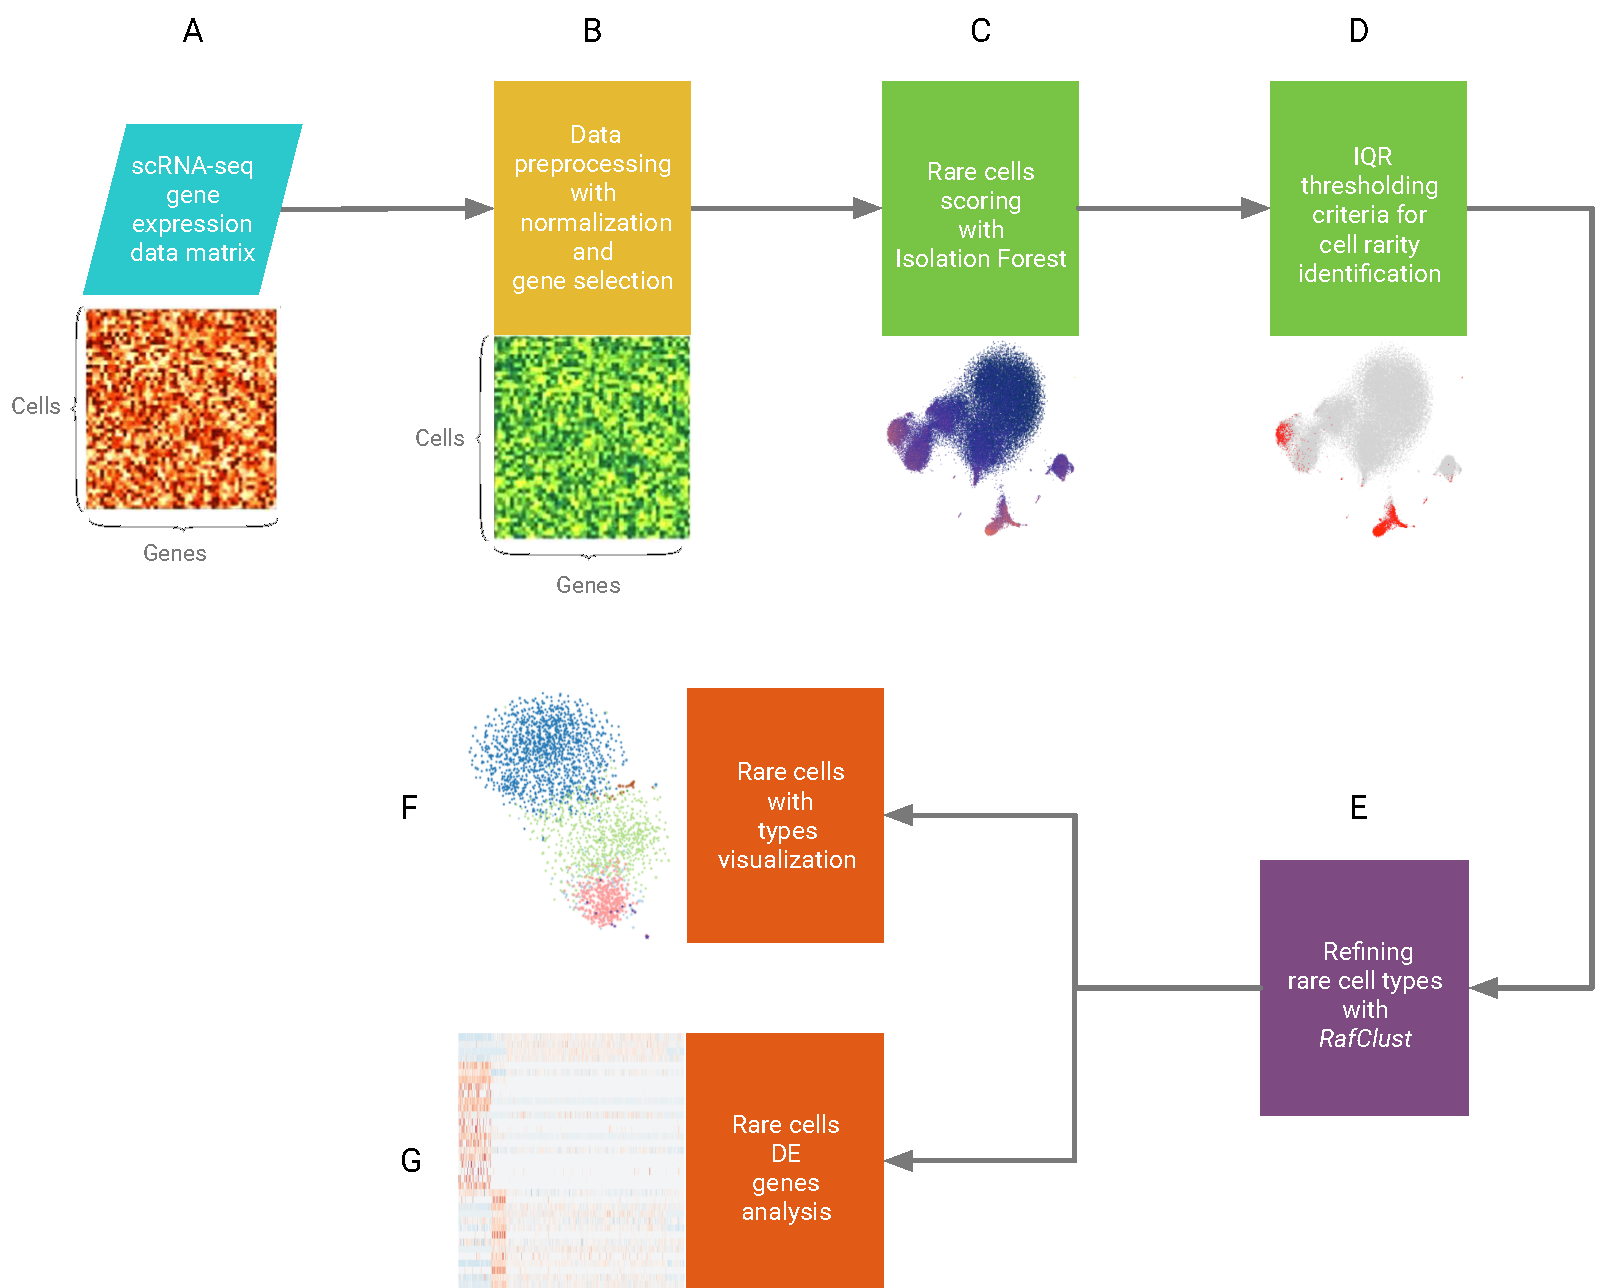
\includegraphics[width=0.95\textwidth]{flowchartv4.pdf}
    % \caption{DoRC flowchart. The flowchart illustrates the processes of our proposed DoRC method for rare cells detection from ultra-large scRNA-seq data. 
    % Each annotated vignette in this figure represents the input or output visualization for the corresponding procedure. 
    % (A) The input is the scRNA-seq expression data 2D-matrix, whose row stands for cells, column for genes, respectively.
    % (B) Data preprocessing with the input expression data, the output is  a normalized and the column dimension reduced matrix. 
    % (C-D) Rare cells discovery with Isolation Forest, which are the workhorse procedures of DoRC. 
    % (C) Rare cells scoring with Isolation Forest, the output is a list of continuous anomaly scores for all the cells.
    % The scores can be visualized in the t-SNE-based 2D plot of the dataset; 
    % (D) IQR thresholding criteria for cell rarity identification, the binary annotations are also visualized in the t-SNE-based 2D plot.
    % (E) Refining rare cell types with RafClust. Notably, this sub-procedure is optional if we do not care about the types of rare cells.
    % (F) Rare cells with types visualization, different colors represent different rare cell types in the t-SNE-based 2D plot of the rare cells.
    % (G) Different expression genes analysis with different types of rare cells, the cell type specific genes are consequently obtained. 
    % }
    \caption{DoRC~流程图。该流程图展示了我们提出的从超大规模~scRNA-seq~数据中检测稀有细胞的过程。
    本图中的每个注释图代表了相应过程的输入或输出可视化。
    (A)~输入的是~scRNA-seq~表达数据二维矩阵,其中行代表细胞,列代表基因。
    (B)~用输入的表达数据进行数据预处理,输出的是一个归一化和列的维度缩减的矩阵。
    (C-D)~用~Isolation Forest~发现稀有细胞,这是~DoRC~的核心程序。
    (C)~用~Isolation Forest~进行稀有细胞评分,输出的是所有细胞的连续的异常得分向量。
    分数可以在基于~t-SNE~的数据集二维图中可视化。
    (D)~细胞稀有度识别的~IQR~阈值标准,二元标注也可以在基于~t-SNE~的二维图中可视化。
    (E)~用~RafClust~确定稀有细胞类型。值得注意的是,如果我们不关心稀有细胞的类型,这个步骤就不需要。
    (F)~稀有细胞与类型可视化,在基于~t-SNE~的稀有细胞二维图中不同的颜色代表不同的稀有细胞类型。
    (G)~对不同类型的稀有细胞进行不同的差异基因分析,从而得到细胞类型的特异基因。
    }
    \label{fig:flowchart}
\end{figure}

\subsubsection{数据规范化和基因选择}
\label{subsec:datapreprocessing} 
每个数据集上,在至少~3~个细胞中读数超过~2~的基因被保留用于下游分析,
然后使用中位数归一化。
除~\textit{Splatter\_500}~之外的其它数据集,
我们基于基于它们的相对分散度~(dispersion,即方差/均值)~与具有相似平均表达量的基因之间的预期分散度~\cite{zheng2017massively,macosko2015highly}选出~1000个变化最大的基因。
最后,将处理后的伪计数矩阵~(pseudo-count)~加~1~后进行对数变换。

\subsubsection{使用孤立森林识别稀有细胞}
\label{subsec:if} 

孤立森林是一种无模型算法,它的计算效率很高,非常适合并行计算方法的使用~\cite{hariri2018batch}。
事实证明,它在检测异常方面也是非常有效的~\cite{susto2017anomaly}。
该算法的主要优越性在于,它并不依赖于为数据设置复杂的参数配置。
相反,它利用了异常数据``少而不同"的特点。
其它大多数异常检测算法~(anomaly detection algorithms)~都是通过了解异常数据的属性分布,并将其从其它正常数据样本中分离出来,从而找到异常数据~\cite{noto2010anomaly,chen2011ordinal,das2016incorporating}。
在孤立森林中结合树结构,从数据中抽取子样本,
并根据数据集中随机选取的特征值进行随机切割。
树枝路径越长,那么该样本为异常样本的可能性越低;
相反,路径越短的树枝越有可能是异常的。
因此,每个树枝的总长度可以被看作是对指定点的异常性衡量的``异常得分"。

孤立森林~\cite{liu2008isolation,liu2012isolation}~的算法思想同任何基于树结构的聚合~(ensemble)~方法一样,
也是在基于决策树结构之上的。
在训练时,给定一个维度为~$N$~的数据集,
该算法选择一个随机的数据子样本来构建一棵二叉树。
树的分支过程通过选择一个随机维度~$x_i$,也就是一个单一的变量或特征来进行,其中~$i \in {1,2,\ldots,N}$。
如果一个给定的数据点在维度~$x_i$~的值小于~$v$,~$v$~是该维度中在最小值和最大值之间的随机值,
那么这个点就会被送到左分支;否则,就会走到右分支。
通过这种方式,树节点当前的数据被分割成两个子数据集。
这个分支过程在数据集上递归执行,直到一个点被隔离,或者达到预定的深度限制。
这个过程再次开始,用一个新的随机子样本来建立另一棵随机化树。
在建立大量的树的集合后,也就是一片森林,训练的过程就完成了。
在评分时,可以使用新的候选数据点或用于创建树的现有数据点。
根据指定点在每棵树中达到的深度,聚合的异常得分的计算式是:
\begin{equation}
    \label{as}
    s(x,n) = 2^{-E(h(x))/c(n)}
\end{equation}
其中, $E(h(x))$~是单个数据点~$x$~在所有树中达到的深度的平均值, $h(x)$~代表~$x$~在树中的深度~(高度)。 
$c(n)$~是归一化因子,定义为二叉搜索树~(BST)~中搜索失败的平均深度。
\begin{equation}
    \label{lab:as}
    c(n) = 2H(n - 1) - (2(n - 1)/n)
\end{equation}
其中~$H(i)$~为谐波数,
可由~$ln(i)~+~0.5772156649$~(欧拉常数)~\cite{liu2012isolation}估计,$n$~为建树时所用的数据点数。
$s(x,n)$~的值接近~1~表示异常,远小于~0.5~表示正常观测值。
我们在这里使用的参数默认值与~\cite{liu2008isolation,liu2012isolation}一样,
即在所有实验中子样本数据为~256,树的集合数目为~100。

虽然异常得分用连续值来表示十分有意义,但有时关于细胞稀有度的二元标注可以极大地简化分析流程~(pipeline)。
因此,如果一个细胞的~DoRC~得分,即聚合异常得分,大于~$q_3 + 1.5 \times IQR$,则~DoRC~将其标记为罕见,
其中~$q_3$和~$IQR$~分别表示所有细胞中~DoRC~分数的第三分位数和四分位数范围(第~75~百分位数$-$第~25~百分位数)。

\subsubsection{差异基因分析}
\label{subsec:de}

使用上一章中介绍的单细胞聚类方法~RafClust~得到了细胞的类别标签后,
我们采用~NODES~\cite{Sengupta049734}~这一快速的非参数化、差异化表达~(DE)~分析工具进行差异基因分析。
NODES~被证明比传统的基于批量细胞测序的差异分析方法~DESeq2~\cite{love2014moderated}、edgeR~\cite{robinson2010edger},
以及针对单细胞的差异表达分析方法~scde~\cite{kharchenko2014bayesian}~和~Wilcoxon~秩和检验~(Wilcoxon rank sum test)~都有效~\cite{Sengupta049734}。
以~0.05~作为~FDR~(False Discovery Rate)~的阈值,~FC~(fold change)~变化(也就是两个组间表达量的比值)~阈值默认为~log2(5)。
在~DE~基因中,在特定类中相对于其余各类显著上调的基因被命名为细胞类型特异基因。


\subsection{实验结果}

\subsubsection{数据集}
\label{subsec:datasets} 

第一个数据集~\textit{PBMCs\_68k}由~68579~个从健康供体收集的~PBMCs~组成~\cite{zheng2017massively}。
11~个纯化的~PBMCs~亚群的单细胞表达谱被用作细胞类型标签的参考。
该数据集可在~\url{www.10xgenomics.com}~下载。

%第二个数据集textit{MSE/20k}包含了来自小鼠大脑Arc-ME区域周围的~${sim} 20$k scRNA-seq图谱~\cite{campbell2017molecular}。
%作者将神经元细胞分为34个簇。
%和非神经元细胞通过二传聚类方法分为30个聚类。
%我们只关注30个非神经元集群,其中包括8092个非神经元细胞。
%数据集~(GSE93374)~是从\url{https://hemberg-lab.github.io/scRNA.seq.datasets/mouse/brain/}下载的。

第二个数据集~\textit{Jurkat\_293T}~是由~Jurkat~和~293T~的两个表达谱构建的,同样来自同一研究~\cite{zheng2017massively}。
Jurkat~数据集由~3258~个细胞组成,而~293T~数据集由~2885~个细胞组成。
首先,从~293T~数据集中不放回抽样~1500~个细胞。
然后,通过从~Jurkat~数据集中取样不同数量的细胞,
产生~8~个数据集,其中~Jurkat~细胞数占比分别为~0.5\%、1\%、1.5\%、2\%、2.5\%、5\%、10\%、15\%。
这两个数据集的表达矩阵也可以从~\url{www.10xgenomics.com}~下载。

最后一个数据集~\textit{Splatter\_500}~是一个人工仿真~scRNA-seq~数据,
通过使用~R~包~Splatter~\cite{zappia2017splatter},由~500~个细胞组成。
与两种细胞类型:~25~个细胞是罕见的~(也就是~rare cells),其它~475~个细胞是丰富的~(也就是~abundant cells)。
在这个数据集中,每个细胞有~5000~个基因。
在~R~中我们使用下面的命令来生成这个数据集:

\texttt{splatSimulate(group.prob = c(0.95, 0.05), method = groups, 
verbose = F, batchCells = 500, de.prob = c(0.4, 0.4), out.prob = 0, 
de.facLoc = 0.4, de.facScale = 0.8, nGenes = 5000)}

\subsubsection{评价指标}

在两类实验中,直接构建一个混淆矩阵~(confusion matrix),其数字为真阳性~(TP)、假阳性~(FP)、真阴性~(TP)、假阴性~(FN)。
混淆矩阵上的精确性、召回率和~F1-score~可以很容易地计算如下:
\begin{equation}
    \label{eq:precision}
    \text{Precision} = \frac{\text{TP}}{\text{TP} + \text{FP}}
\end{equation}
\begin{equation}
    \label{eq:recall}
    \text{Recall} = \frac{\text{TP}}{\text{TP} + \text{FN}}
\end{equation}
\begin{equation}
\label{eq:f1score}
\text{F1-score} = 2 \times \frac{\text{Precision} \times \text{Recall}}{ \text{Precision} + \text{Recall}}
\end{equation}
在模拟实验中,对于其~DoRC~分数满足~IQR~阈值的标准的被认定为是稀有细胞。
对于实验中采用的~\textit{Jurkat\_293T}~数据集,计算出~Jurkat~细胞的~F1~分数。

\subsubsection{实验结果分析}

%\subsubsection{DoRC~概览}
\label{subsec:dorc}
RaceID~和~GiniClust~都依靠无监督聚类来检测稀有细胞。
RaceID~中的~\textit{k}-means~聚类是基于距离的,
而~GiniClust~中的~DBSCAN~聚类是基于密度的。
它们都属于基于近邻的方法进行离群点检测。
基于近邻的方法假设一个离群物体与其最近邻居的接近程度与该物体与数据集中大多数其它物体的接近程度有很大的差异。
聚类通常取决于一些敏感参数且工作效率低下,因为不同分布的数据点之间的近似度不同。
另一个主要问题是决定群体身份的解析。
一般来说,多级聚类变得至关重要,因为次要的类经常在首次筛选就被忽略~\cite{campbell2017molecular}。
发生这种情况是因为其它主要细胞类型会影响数据集中的表达差异,
特别是在处理大型~scRNA-seq~数据集时,情况变得更加糟糕。

为了解决上述问题,我们提出了一种从超大规模~scRNA-seq~数据中检测稀有细胞的非常快速的方法,
命名为~DoRC。
DoRC~的灵感来自于我们观察到稀有细胞在单细胞数据集里往往是``少而不同", 这跟机器学习里的样本孤立特性十分相似。
孤立森林可以充分捕捉稀有细胞的特征,
其中,每个细胞的稀有性是以树枝的聚合长度为特征的。
一个细胞的长度越长,该细胞与其它细胞区分的因素就越多,它成为稀有细胞的可能性就越大。
从数量上看,孤立森林中的聚合异常分数在本质上反应了稀有特性,
这为我们调查和进一步决定细胞的稀有性提供了基础。
为了说明这一点,我们将~DoRC~应用于包含~${\sim}68$k~外周血单核细胞的~scRNA-seq~数据集~(PBMCs)~的标注进行比对,
这个数据集是知名的纯化的免疫细胞亚型数据集~\cite{zheng2017massively}。
研究者首先对细胞进行了无监督聚类,
然后根据之前已知的标记对类进行注释~(图~\ref{supp-fig:dorcsummary} A)。
我们将~DoRC~的分数叠加在这一个二维图上~(图~\ref{supp-fig:dorcsummary} B)。
最高~0.1\%~的~DoRC~分数对应的是最小的, 
清晰地标注了含有巨核细胞的~CD34+~类别~(图~\ref{fig:dorcsummary} A)。
据报道,巨核细胞只含有整个细胞集的~0.3\%~\cite{zheng2017massively}。
然后,我们将这一比例从~0.1\%~增加到~1.0\%,随后又增加到~3.0\%,
然后下一批次的细胞亚型被选入扩展的稀有细胞集合中。
这些细胞包括单核细胞和树突状细胞亚型的亚类~(图~\ref{fig:dorcsummary} B-C)。
这个案例研究展示了~DoRC~在检测不同比例的稀有细胞方面的表现。

\begin{figure*}[!htbp]
    \centering
    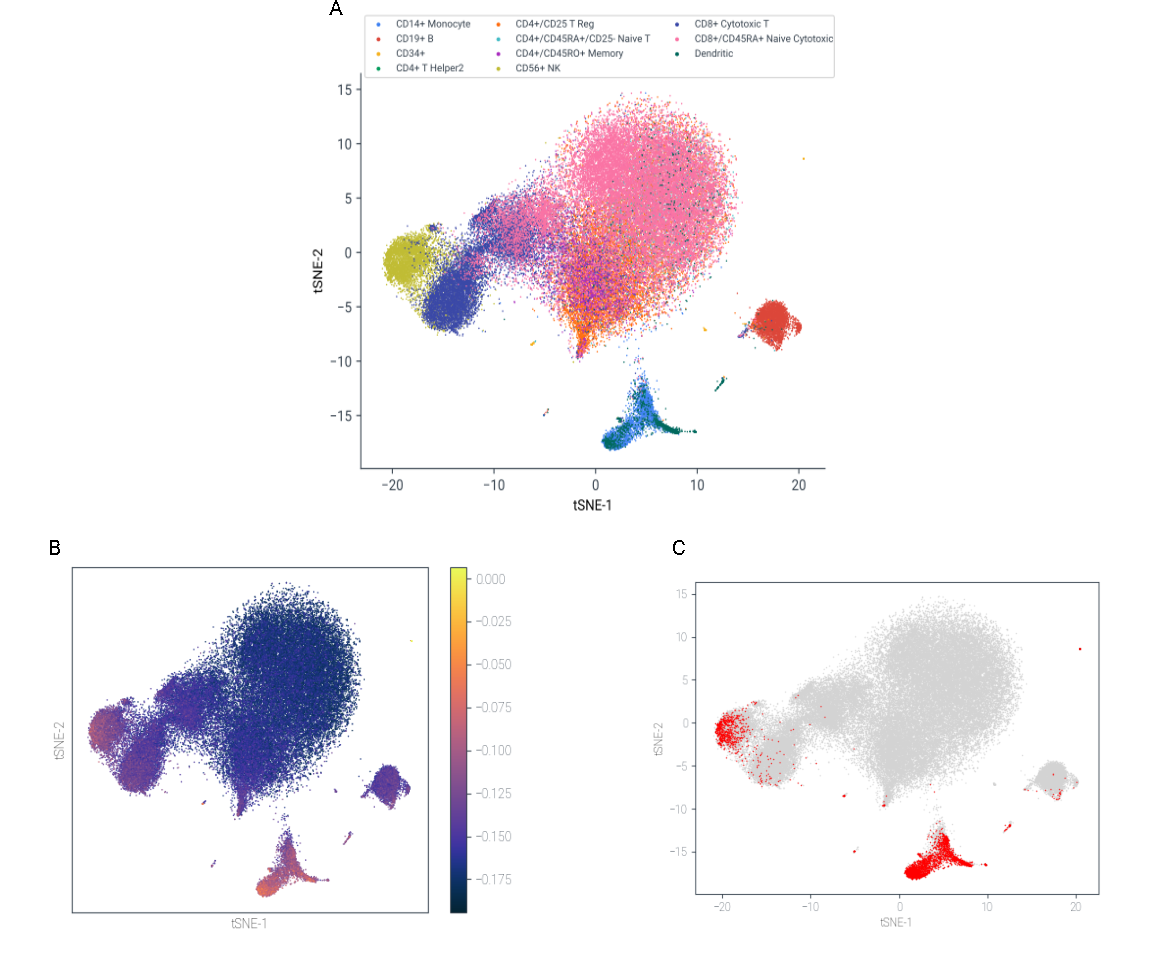
\includegraphics[width=0.9\textwidth]{DoRCSummarySI.pdf}
    \caption{
    % Performance evaluation of DoRC on PBMCs\_68k. 
    % (A) t-SNE based 2D embedding of the data with color-marked cluster identities as reported by Zheng et al.~\cite{zheng2017massively}. 
    % (B) Heat map of DoRC scores for the cells on PBMCs\_68k. 
    % The cluster of megakaryocytes (0.3\%), the rarest of all the cell types are assigned the
    % highest DoRC scores.
    % (C) Rare cells identified by DoRC using IQR-thresholding-criteria
    DoRC~在~PBMCs\_68k~上的性能评估。
    (A)~基于~t-SNE~的二维嵌入数据集可视化图,按~Zheng~等所报道的鉴定的不同类别用不同的颜色标记。
    (B)~PBMCs\_68k~上细胞的~DoRC~得分热图。巨核细胞群~(0.3\%),是所有细胞类型中最稀有的细胞,获得了最高的~DoRC~分数。
    (C)~使用~IQR~阈值标准后~DoRC~识别的稀有细胞。
    }
    \label{supp-fig:dorcsummary}
\end{figure*}

\begin{figure*}[!htbp]
    \centering
    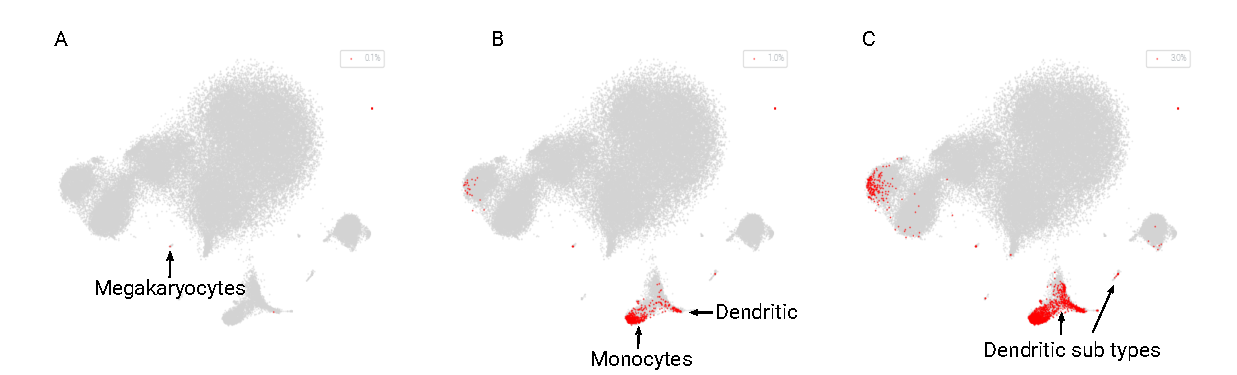
\includegraphics[width=0.9\textwidth]{DoRCSummary.pdf}
    \caption{
    % DoRC discovers cells with varying degrees of rarity. In the ${\sim}68$k PBMC data~\cite{zheng2017massively}, minor cell populations with different grades of rarity show up with an
    % increase in the number of selected rare cells. (A-C) The top 0.1, 1.0 and 3.0\% cells, respectively, selected on the basis of DoRC scores are highlighted
    DoRC~发现了不同稀有度的细胞。在~${\sim}68$k~PBMC~数据~\cite{zheng2017massively}~中,不同级别的稀有度对应了一个数量不断增加的稀有细胞群。
    (A-C)~根据~DoRC~得分选出的前~0.1\%、1.0\%~和~3.0\%~的细胞分别以高亮显示。    
    }
    \label{fig:dorcsummary}
\end{figure*}

虽然连续的分数是有意义的,
如果能对细胞稀有性给出二元标注~(binary annotations),则有助于简化后续分析。
为了解决这个问题,我们引入了一个基于得分分布特性的阈值方法。
图~\ref{supp-fig:dorcsummary} C~显示了~${\sim}68$k~PBMC~数据中检测到的细胞。
我们利用基于阈值的二分法来标注稀有细胞,
如预期的那样,
大部分检测到的稀有细胞来源于已知的次要细胞类型,包括巨核细胞、树状细胞和单核细胞,
如图~\ref{supp-fig:dorcsummary} A~上所示的分别对应于~CD34+、树枝状和~CD14+~单核细胞。


%\subsubsection{DoRC~揭示了树突状细胞之间的异质性}

树突状细胞~(DC)~在感知、吞噬和和抗原监视~\cite{villani2017single}~方面起着至关重要的作用。
DCs~是最罕见的免疫细胞类型之一,在~PBMCs~\cite{zheng2017massively}~数据集上占比约~0.5\%。
Villani~\cite{villani2017single}~的研究划分了六种不同的树突状细胞的亚型。
他们通过荧光激活细胞分选~(FACS)~来分析了树突状细胞、分型~DCs~和单核细胞的表达。
他们在研究中报告的~DC~亚型如下:
$\text{CD141}^+$~DCs~(DC1), 
$\text{CD1C}^+${\_}A~常规~DCs~(DC2),
$\text{CD1C}^+${\_}B~常规~DCs~(DC3),
$\text{CD1C}^-\text{CD141}^-$(DC4),~DC5~和浆细胞~DCs~(DC6,pDCs)。

我们很好奇树突状细胞亚型是否可以在~PBMCs~数据中被准确识别。
首先,我们在~${\sim}68$k PBMCs~数据集上应用~DoRC。
DoRC~通过使用基于~IQR~的二分法,共发现了~3844~个稀有细胞。
然后通过~RafClust~对稀有细胞进行聚类~(见~\ref{subsec:rafclust}),得到~12~个子类别。
在这~12~个可区分的聚类中~(C0-C11),
C4、C5、C9~和~C11~完全由树枝状细胞组成,根据~Zheng~等人提供~\cite{zheng2017massively}的标注,
如图~\ref{fig:dorc_dendritic} A-C~所示。
对于这~4~个~DC~类别,我们进行差异表达分析,找出细胞类型特异性基因~(见~\ref{subsec:de})。
共有~21~个基因被检测为细胞类型特异性基因,使用阈值为~log2(1.5)~的~FC~(fold change)。
通过将我们的差异基因与~Villani~\cite{villani2017single}~报道的基因进行叠加。
我们可以有信心地解析~6~个亚型中的~5~个~(DC1、DC2、DC4、DC6)~(图~\ref{fig:dorc_dendritic} D、表~\ref{supp-tbl:dendritic})。
从~\cite{villani2017single}~可以看出,~DC5~是未识别的~(unresolved)~的,因为该类型是新分离出来的罕见类型。
在~t-SNE~二维嵌入图中,~DC3~与~DC2~属于同一类~\cite{maaten2008visualizing}。
在~DoRC~检测到的稀有细胞上使用~RafClust~进行聚类,不能完全划分出树突状细胞亚型正确的数量。
然而,在最初~\cite{zheng2017massively}的研究中,~DC1~和~DC4~也没有被聚类算法识别到。
事实上,在原始文献~\cite{zheng2017massively}~的t-SNE~图中,
这些细胞类型在视觉上共同聚集在自身或单核细胞内。
\begin{figure}[!htbp]
    \centering
    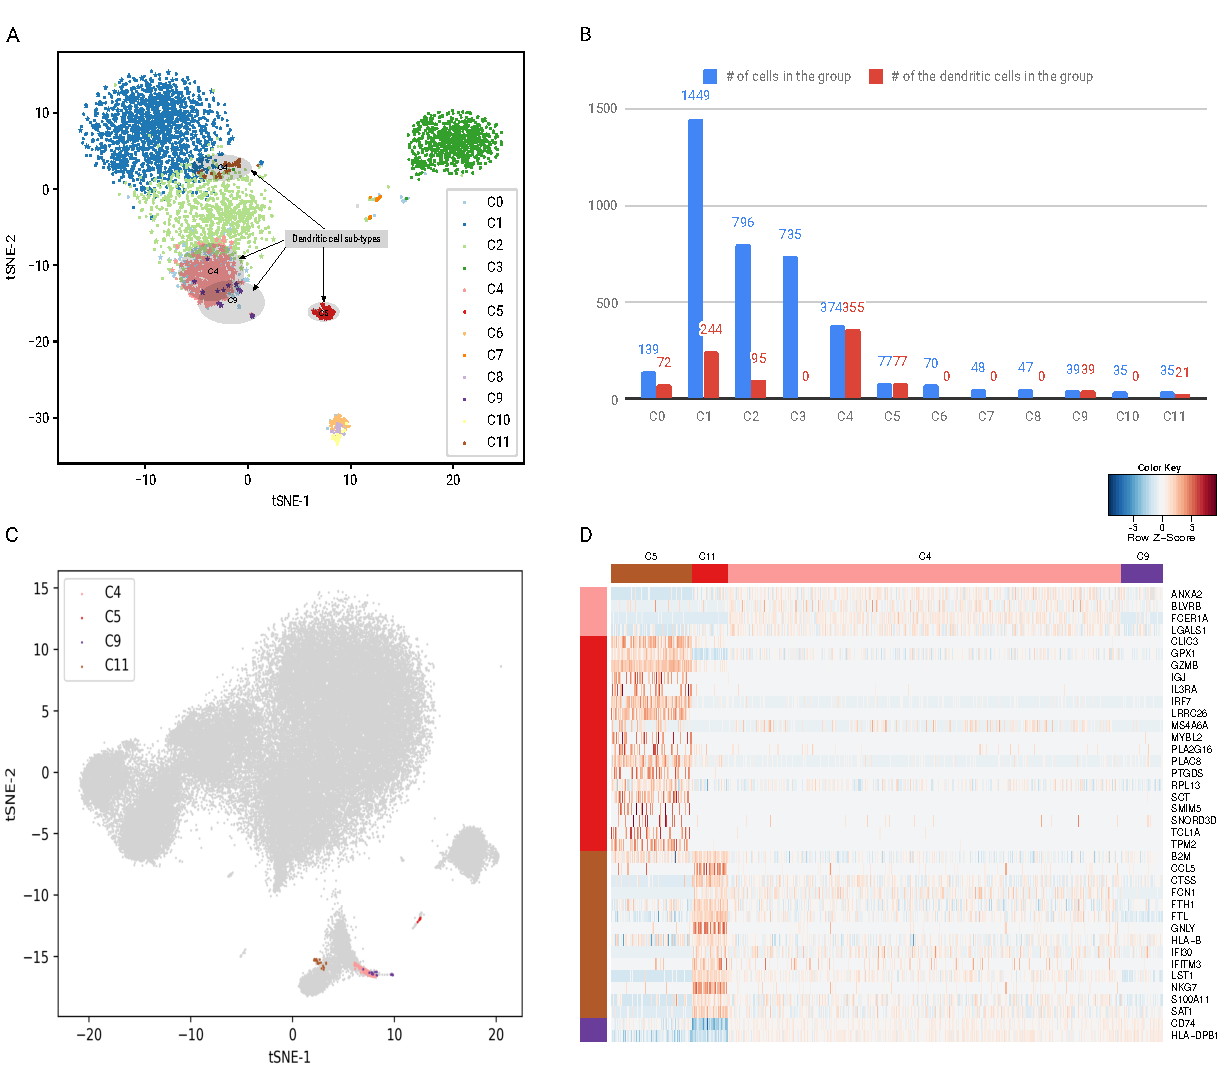
\includegraphics[width=0.9\textwidth]{plot_tsne_dorc_rare_summary.pdf}
    \caption{
    % Human blood dendritic cell heterogeneity delineated by DoRC. 
    % (A) DoRC detected rare cells are clustering into 12 sub types with RafClust, 
    % i.e.~C0 (a singleton class), C1, $\ldots$, C11.
    % With the annotation given by~\cite{zheng2017massively}, C4, C5, C9, C11 are mostly dendritic cells sub types.
    % Dots with the same color represent one subpopulation by clustering the rare cells with RafClust.
    % For each subpopulation, the cells annotated with asterisks marking are also dendrotic cells according to the annotation given by~\cite{zheng2017massively}. 
    % (B) The cells number for each subpopulation and the number of dendrotic cells in this group. 
    % Apparently, dendritic cells hold the majority of the subpopulation in C4, C5, C9, C11.
    % (C) These four dendritic sub-types cells are highlighted on the~\textit{PBMCs\_68k} dataset t-SNE-based 2D plot.
    % (D) Characterization of dendritic cell sub-types utilizing markers obtained from DE analysis (See~\ref{subsec:de})
    DoRC~检测到人类血液树突状稀有细胞的异质性。
    % (A)~DoRC~检测到的稀有细胞在~RafClust~中被聚成~12~个亚型,即~C0,C1,$\ldots$,C11。
    % 通过~\cite{zheng2017massively}~给出的标注,~C4、C5、C9、C11~多为树枝状细胞亚型。
    % 用~RafClust~聚类稀有细胞,同种颜色的点代表一个亚群。
    % 对于每个亚群,根据~\cite{zheng2017massively}~给出的注释,
    % 用星号标记的细胞也是树突状细胞。
    % (B)~每个亚群的细胞数和本组中树突状细胞的数量。
    % 显然,树枝状细胞在~C4、C5、C9、C11~的亚群中占有多数。
    % (C)~这四种树枝状亚型细胞在~\textit{PBMCs\_68k}~数据集的~t-SNE~二维图上突出显示。
    % (D)~利用从~DE~分析中获得的标记来描述树突状细胞亚型的特征~(见节~\ref{subsec:de})
    }
    \label{fig:dorc_dendritic}
\end{figure}

\begin{table}[!htbp]
    \centering
    \caption{
        %The dendritic cell types correspond to class types reported by Villani~\cite{villani2017single}
        树枝状细胞类型对应于~Villani~报告的细胞类别~\cite{villani2017single}
        }
    \label{supp-tbl:dendritic}
    \resizebox{\columnwidth}{!}{
    \begin{tabular}{clc}
    \hline
    Class type & \multicolumn{1}{c}{Marker gene(s)}                                                                                                                                   & Corresponding class type \\ \hline
    C4         & ANXA2, BLVRB, \textbf{FCER1A}, LGALS1	                                                                                                                                         & DC2                      \\ \hline
    C5         & \begin{tabular}[c]{@{}l@{}}CLIC3, GPX1, \textbf{GZMB}, \textbf{IGJ}, \textbf{IL3RA}, \textbf{IRF7}, LRRC26, MS4A6A, MYBL2,\\ PLA2G16, PLAC8, PTGDS, RPL13, SCT, SMIM5, SNORD3D, TCL1A, TPM2\end{tabular} & DC6                      \\ \hline
    C9         & \begin{tabular}[c]{@{}l@{}}B2M, CCL5, CTSS, FCN1, FTH1, \textbf{FTL}, GNLY, HLA-B, IFI30, \textbf{IFITM3}, \textbf{LST1},\\ NKG7, S100A11, SAT1\end{tabular}                                    & DC4                      \\ \hline
    C11        & CD74, \textbf{HLA-DPB1}                                                                                                                                                       & DC1                      \\ \hline
    \end{tabular}
    }

    \begin{tablenotes}
        \small
        %\item Note: Those genes marked in bold are acting as  marker genes in the corresponding class type.
        \item 注:~用粗体标记的基因在相应的类型中起着标志~(Marker)~基因的作用。
      \end{tablenotes}

\end{table}

% \subsubsection{DoRC~能够识别人工伪造的稀有细胞}
\label{subsec:recplanted} 
我们设计了一个模拟实验来评估~DoRC~在细胞类型识别上的性能表现。
我们使用了一个~scRNA-seq~数据集~Jurkat\_293T,由~293T~和~Jurkat~细胞在体外以不同比例混合组成~(见节~\ref{subsec:datasets})。
作者利用每个细胞的单核苷酸变异~(SNV)~谱来确定其系谱。
我们认为这种基于基因型的标注接近真实的细胞标签。

随着~Jurkat~(稀有)~细胞在所有细胞中的占比变化,比例从~0.5\%~到~15\%,
我们得到~8~个数据集。
对于每个数据集,~F1-score~是用通过~DoRC~评分和~IQR~阈值标准确定预测标签,然后与两个类的真实标签进行计算。
重复这个过程~100~次,可以得到该数据集的~F1~分数的标准差。
标准差反应了该方法识别人工伪造的稀有细胞的稳定性~(图~\ref{fig:jurkat} A)。 
F1-score~反应了精度和灵敏度之间的平衡。
当稀有率处于低水平时,即~0.5\%~和~1\%~时,~DoRC~无法匹配~FiRE。
但是,当稀有率从~1.5\%~增加到~15\%~时,~DoRC~的性能优于~FiRE。
此外,~FiRE~的性能在~15\%~的稀有率下急剧下降,但是~DoRC~更保守,性能损失较小。

特别地,在上述~8~个数据集中,我们选取了稀有细胞占比为~2.5\%~时的对应的数据集作为基准数据集。
%从~100~个生成的数据集中随机选取了一个有~1539~个细胞的混合数据集,作为基准数据集。
从~t-SNE~图~\ref{fig:jurkat} B~上可知,该数据集上~39~个稀有细胞和~1500~个丰富细胞非常清晰地聚成两组。
在~FiRE~和~DoRC~这两种方法中,稀有细胞的得分都清晰地高于丰富细胞类型~(图~\ref{fig:jurkat} C-D)。
每种方法都得到了二元标签~(图~\ref{fig:jurkat} E-F),~DoRC~的表现优于~FiRE,
因为它有更好的能力来检测更多的稀有细胞~(图~\ref{fig:jurkat} G-H)。

\begin{figure}[!htbp]
    \centering
    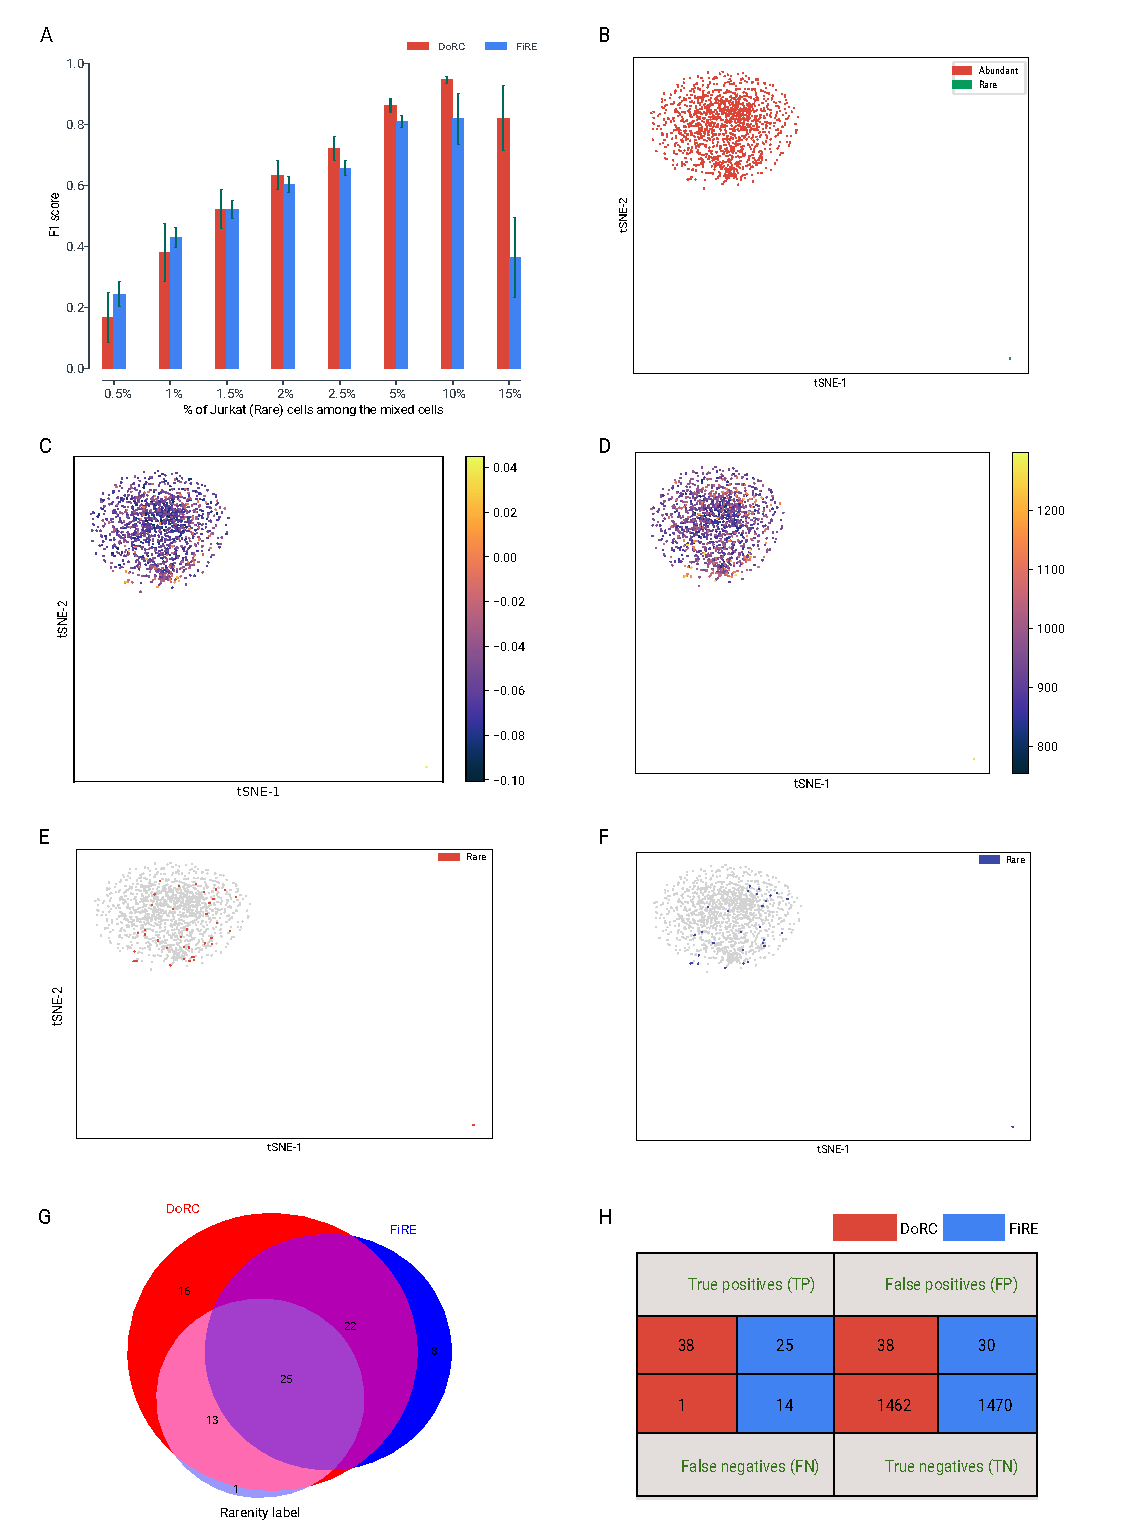
\includegraphics[width=0.9\textwidth]{plot_venn_dorcfire_39summary_compressed.pdf}
    \caption{
    % Detectability of minor cell types in a simulated dataset consisting of Jurkat and 293T cells. 
    % (A) The F1-scores are calculated w.r.t. the rare (Jurkat) population for DoRC and FiRE, 
    % while bioinformatically varying the proportion of artificially planted rare cells.
    % (B) The t-SNE-based 2D embedding of the cells with color-coded identities of the benchmark dataset.
    % (C-D) DoRC and FiRE score intensities plotted on the t-SNE-based 2D map, respectively. 
    % (E-F) The rare cells detected by DoRC and FiRE, respectively, are highlighted.
    % (G) DoRC, FiRE detected rare cells and true rare cells overlap with each other, shown in this Venn diagram. 
    % (H) Detail of the confusion matrices with TP, FP, FN, TN prediction metrics for DoRC and FiRE.
    在由~Jurkat~和~293T~细胞组成的模拟数据集中,次要细胞类型的可检测性示意图。
    % (A)~按照生物信息上逐渐改变人工植入的稀有细胞的比例,计算关于稀有类别~(也就是~Jurkat)~的~DoRC~和~FiRE~的~F1~分数。
    % (B)~基准数据集上细胞的基于~t-SNE~的二维嵌入可视化图,不同颜色代表不同的细胞类别。
    % (C-D)~DoRC~和~FiRE~得分分别绘制在基于~t-SNE~的二维嵌入可视化图上。
    % (E-F)~DoRC~和~FiRE~分别检测到的稀有细胞,用高亮来显示。
    % (G)~DoRC~和~FiRE~检测到的稀有细胞和真正的稀有细胞相互重叠,在该维恩图中显示出来。
    % (H)~DoRC~和~FiRE~的混淆矩阵与~TP、FP、FN、TN~指标的计算细节。
    }
    \label{fig:jurkat}
\end{figure}

%\subsubsection{DoRC~对细胞类型敏感}

我们设计了一项模拟研究来分析~DoRC~评分的鲁棒性和敏感性与差异表达基因~DE~数量的关系。
我们首先生成一个由~500~个两种细胞类型组成的人工仿真的~scRNA-seq~数据。
数量小的细胞类型约占细胞的~5\%~(见节~\ref{subsec:datasets})~。
我们将通过严格的标准选择的差异表达基因保留在一边。
对于每次实验的迭代,我们将预先确定的~DE~基因附加到固定数量的非~DE~基因上。
我们在~1~和~150~之间改变差异表达基因的数目,来跟踪~DoRC~在检测规模小的类别细胞的敏感性。
随着给定的~DE~基因集合,计算细胞的~DoRC~分数,并对小类别细胞进行计算接收者操作特征曲线~(ROC)~下面积~(AUC)。
对于每一种数量的~DE~基因,上述过程重复~1000~次。
汇总后的平均~AUC,以及所有的~AUC~的标准差如图~\ref{fig:simulate:roc}~中所示。
随着~DE~基因数量的减少,~DoRC~难以检测到次要细胞群。
然而,当引入~20~个或更多的~DE~基因时,~DoRC~的预测率急剧提升。
同时,随着偏差变小,预测变得更加稳定。
另外从~t-SNE~图上可以看到,由于~DE~基因的增加,两类细胞能够更加直观地区分出来。
这个实验反应了~DoRC~对噪声具有一定的鲁棒性。

\begin{figure}[!htbp]
    \centering
    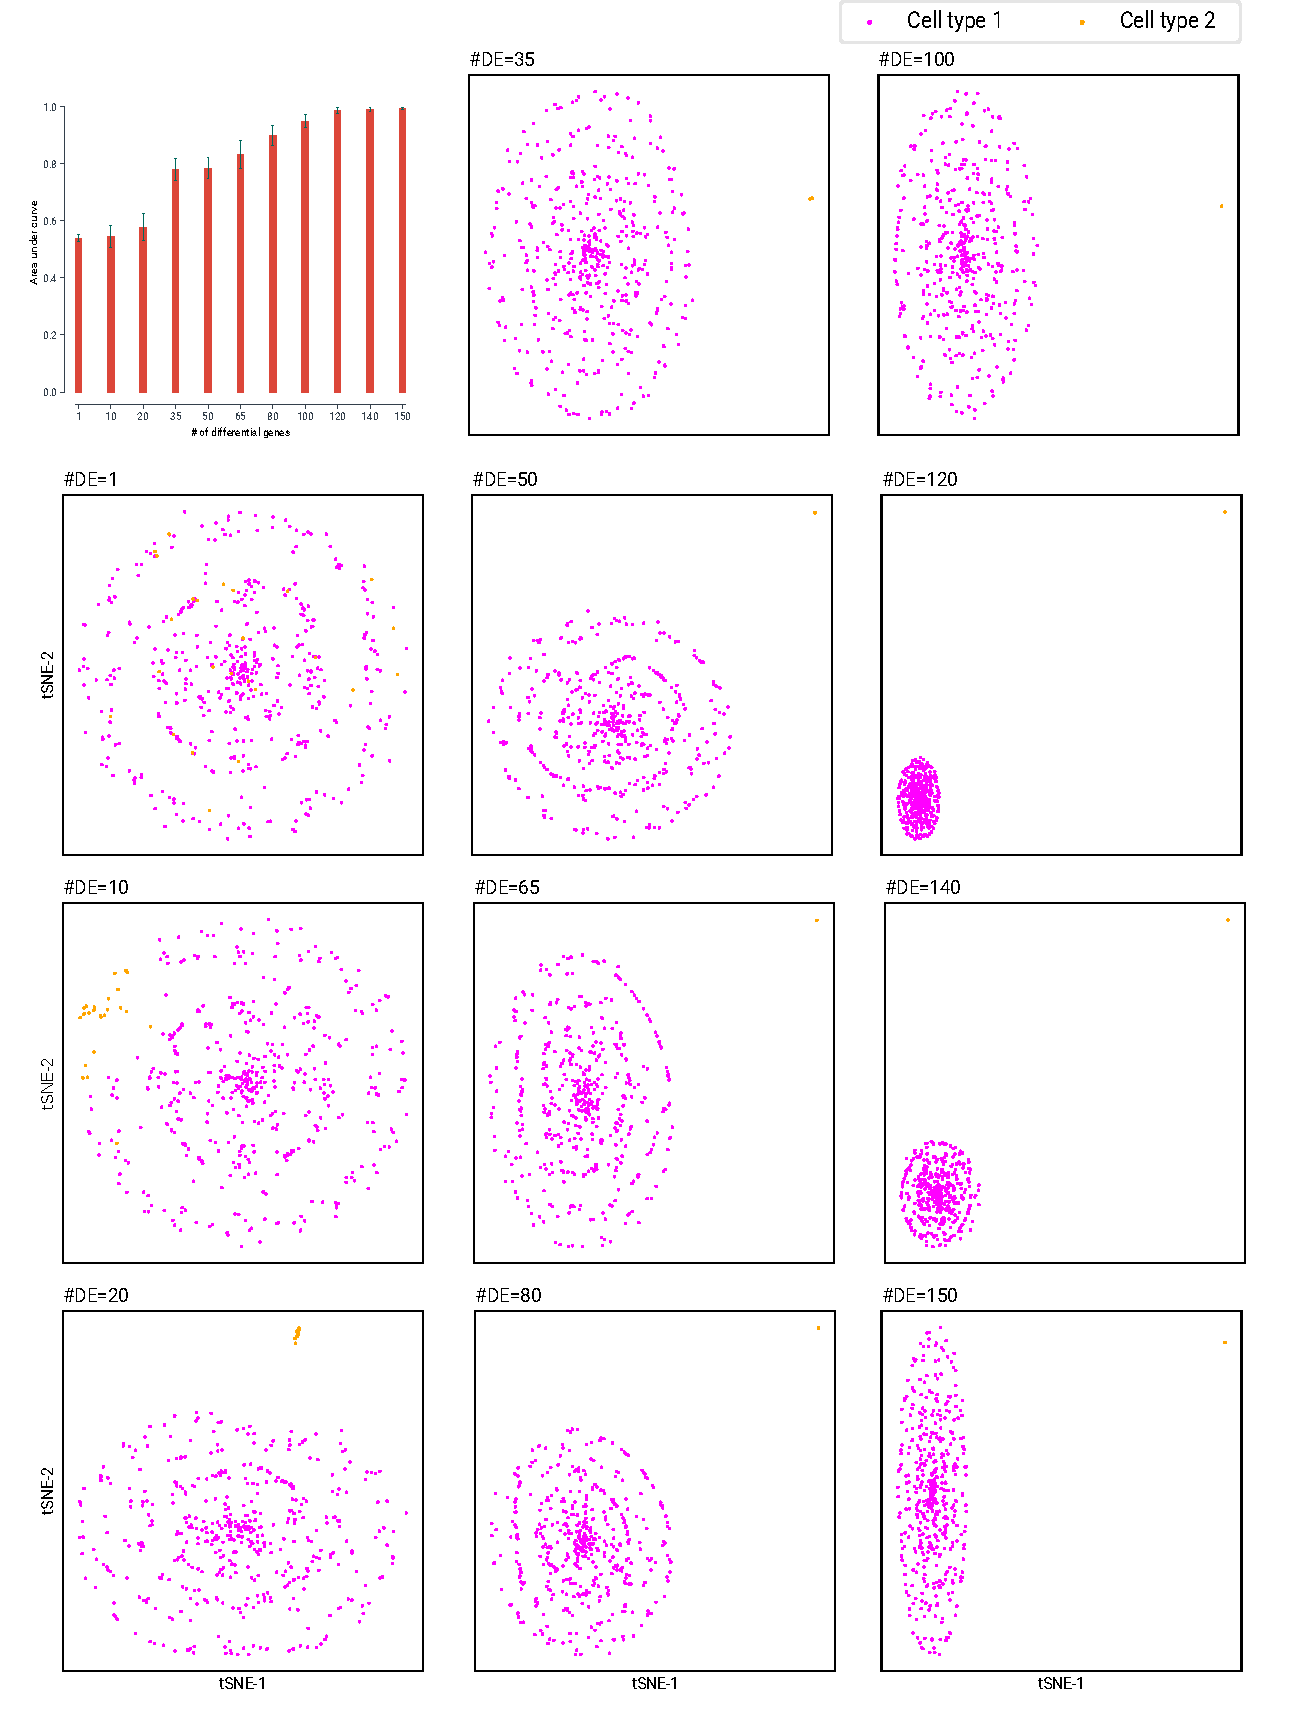
\includegraphics[width=0.9\textwidth]{simulate_panorama.pdf}
    \caption{
    % The sensitivity of DoRC to cell-type identities. 
    % On the scRNA-seq dataset \textit{Splatter\_500}, 
    % DoRC starts with recognizing the minor cell type correctly, 
    % as soon as the number of differentially expressed genes becomes adequate to give rise to a tiny cluster representing the minor cell
    % subpopulation. 
    % The top-left corner figure serves as a legend for the subsequent AUC plots. 
    % Each t-SNE and ROC plot pair serves as a representative of the 1000 repetitions of the experiment concerning a
    % specific number of differentially expressed genes. 
    % The AUC analysis is performed using cell-type annotations, 
    % and DoRC scores are assigned to individual cells.
    DoRC~对细胞类型特征敏感。
    % 在~scRNA-seq~数据集~\textit{Splatter\_500}上,
    % DoRC~从正确识别比例小的细胞类型开始,
    % 只要差异表达基因的数量变得足以产生一个代表小细胞亚群的微小簇。
    % 左上角图作为后续AUC图的图例。
    % 每个~t-SNE~和~ROC~图对对应为为~1000~次重复实验的一个代表结果,
    % 对应于一种特定数量的差异表达基因。
    % AUC~是使用各个细胞的类型标签和~DoRC~得分来计算到的。
    }
    \label{fig:simulate:roc}
\end{figure}

此外,由于~DoRC~和~FiRE~都可以给细胞做二元标注,
我们对其性能差异感到好奇。
在这个数据集中,我们考虑了~DoRC~和~FiRE~之间的~AUC、召回率、精度和~F1-score。
由于~F1-score~取决于召回率和精度,我们也包括这两个指标作为参考。
把细胞类型标注为真实标签,~AUC~是用~DoRC~评分计算的。
而~F1-score是用~DoRC~评分产生的稀有度标注与~IQR~阈值标准获得的。
在总共~25~个稀有细胞中,~DoRC~和~FiRE~都能正确检测出~23~个相同的稀有细胞。
DoRC~可以检测到其它~2~个稀有细胞和~1~个假阳性稀有细胞,
而~FiRE~未能识别出左边~2~个稀有细胞~(图~\ref{fig:simulate:venn_auc_f1} A)。
在这个数据集中, 阳性样品~(丰富细胞)~和阴性样品~(稀有细胞)~的数量是不平衡的。
这两种方法的~AUC~和精度基本没有变化,
但~DoRC~的召回率和~F1-score~均高于~FiRE~(图~\ref{fig:simulate:venn_auc_f1} B)。
\begin{figure}[!htbp]
    \centering
    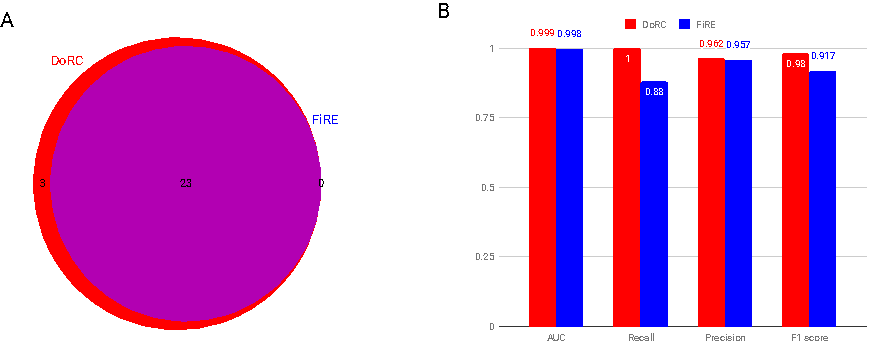
\includegraphics[width=0.9\textwidth]{plot_venn_dorcfire.pdf}
    \caption{
    % Comparison of DoRC and FiRE for rare cells detection in the dataset~\textit{Splatter\_500}.
    % (A) Among all the 25 rare cells,  23 rare cells are all detected by DoRC and FiRE. 
    % DoRC could detect other 2 rare cells and 1 false positive rare cells, 
    % while FiRE failed to identify the left 2 rare cells.
    % (B) The AUC and precision of DoRC and FiRE are almost the same, while the Recall and  F1-score of DoRC is higher than FiRE.
    在~\textit{Splatter\_500}数据集上,~DoRC~和~FiRE~对数据集中稀有细胞检测的比较。
    % (A)~在所有~25~个稀有细胞中,~23~个稀有细胞全部被~DoRC~和~FiRE~检测出来。
    % DoRC~可以检测到另外~2~个稀有细胞和~1~个假阳性稀有细胞,而~FiRE~则未能识别出剩下的~2~个稀有细胞。
    % (B)~DoRC~和~FiRE~的~AUC~和精度几乎相同,而~DoRC~的~Recall~和~F1-score~高于~FiRE。
    }
    \label{fig:simulate:venn_auc_f1}
\end{figure}

%\subsubsection{DoRC~是可扩展和快速的}
%\label{subsec:scalable} 

DoRC~的核心算法孤立森林~(Isolation Forest)~的时间复杂度为~$O(ntlog\psi)$~\cite{liu2008isolation}。
其中~$n$、$t$~和~$\psi$~分别代表样本数、树的数目和每棵树的子样本数。
值得注意的是,~DoRC~中的~Isolation Forest~在这种情况下没有训练的阶段。
该方法的参数我们使用默认值,~t~设置为~100,~$\psi$~设置为~256。
因此,~DoRC~的时间复杂度为~$O(n)$。
这个复杂度没有包括使用~RafClust~来确认稀有细胞的类型,
因为~FiRE~和~LOF~这两种方法也没有包含稀有细胞的类型细化这个步骤。

我们不断变化输入单细胞数据规模的大小,
分别统计出~DoRC、FiRE、GiniClust、LOF~\cite{breunig2000lof}~和~RaceID~所消耗的时间,
如图~\ref{fig:timecomplexity}~所示。
测试机器为一台运行~GNU Linux/Ubuntu 16.04~操作系统~4.15.0-47-generic~内核的工作站上,
硬件配置如下:~Intel(R) Xeon(R) Silver 4116 CPU @ 2.10GHz,~48~核,~64GB~内存。
DoRC~由~Python~实现,使用~scikit-learn包~(版本~0.20.2)~\cite{pedregosa2011scikit}和~pyod包~(版本0.6.7)~~\cite{zhao2019pyod}。
由于其它方法不能区分稀有细胞类型,在~DoRC~中我们也因此省略~RafClust~的稀有细胞类型细化的程序。
FiRE~从~\url{https://github.com/princethewinner/FiRE}~下载~(分支:master,最新提交的~abcba5b)。
因为~FiRE~的内核算法是用~C++~编写的,我们在实验中使用的是其~Python~扩展分支。
GiniClust从~\url{https://github.com/lanjiangboston/GiniClust}~下载~(分支:master,最新提交~a442d45)。
我们在命令行界面直接使用~R~脚本,
额外的步骤包括~t-SNE~可视化和~DE~分析不计入时间对比评测中。
RaceID从~\url{https://github.com/dgrun/RaceID}~下载~(分支:master,最新提交~0a1e21c)。
LOF~(local outlier factor)~是数据挖掘领域应用广泛的算法。
我们也直接使用~Pyod~包~(0.6.7版本)~\cite{zhao2019pyod}~的~Python~实现~LOF。
值得注意的是,~RaceID~和~GiniClust~仅输出了稀有细胞的二分标签预测,
而~DoRC、FiRE~和~LOF~则同时提供连续得分和二分标签预测。
\begin{figure}[!htbp]
    \centering
    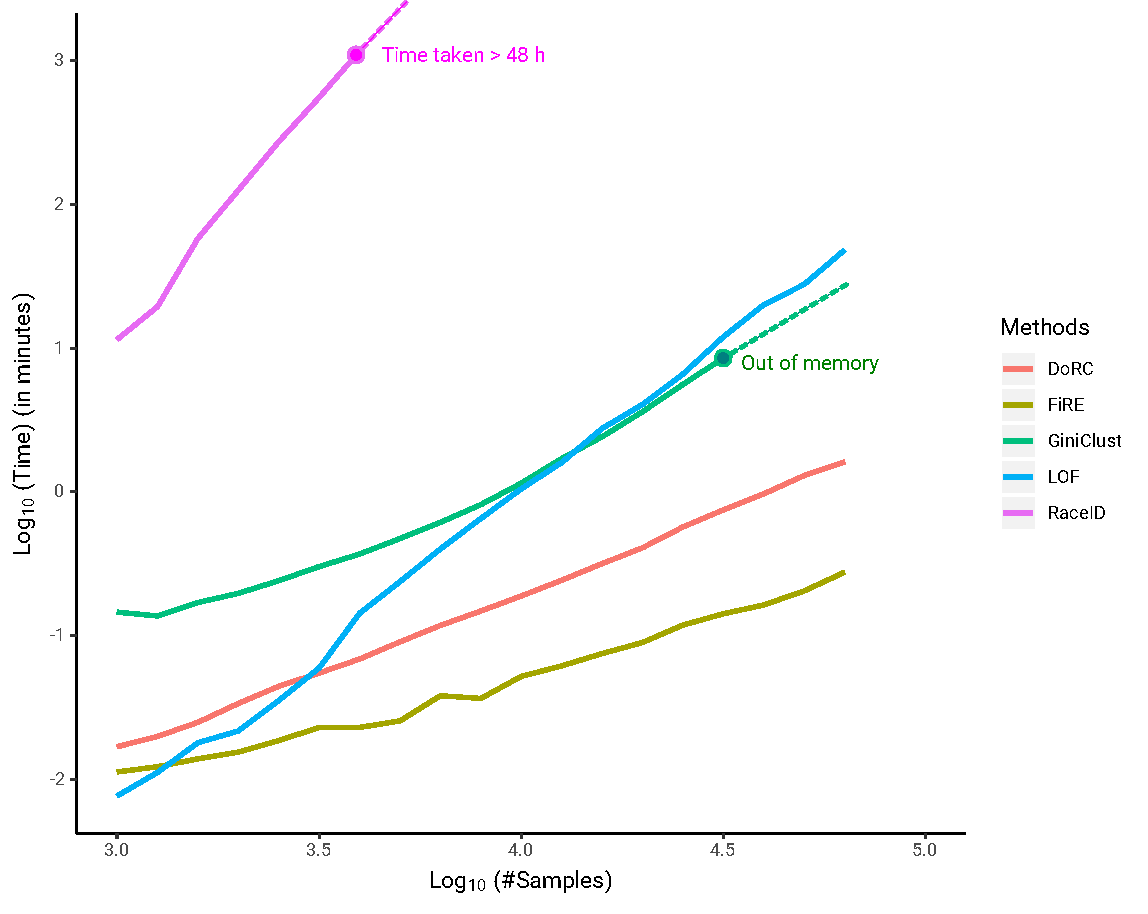
\includegraphics[width=0.9\textwidth]{Rplot_timecomplexity.pdf}
    \caption{
    % DoRC is fast. Execution time is recorded for DoRC, FiRE, GiniClust, LOF and RaceID, while varying the number of cells from 1k to ${\sim} 68$k
    DoRC的执行速度仅次于~FiRE。我们从~1k~到~${\sim} 68$k~逐渐改变细胞的数目, 同时记录下~DoRC、FiRE、GiniClust、LOF~和~RaceID~的执行时间。    
    }
    \label{fig:timecomplexity}
\end{figure}
图~\ref{fig:timecomplexity}~展示了从~${\sim}68$k scRNA-seq~数据中发现稀有细胞不同方法在不同细胞输入规模时所消耗的时间。 
GiniClust~和~RaceID~要么耗时,要么耗内存;
LOF~对输入数据规模非常敏感;
然而,~DoRC~和~FiRE~都是非常快的,因为它们只需要不到~2~分钟就可以完成任务。
与~DoRC~相比,~FiRE~的速度明显更快。
DoRC~的实现代码可在~GitHub~仓库~\url{https://github.com/chenxofhit/DoRC}~上获取,
本章节相关的实验代码和相关数据集可以根据用户的要求提供。

\subsection{讨论和结论}
近来,单细胞转录组学大大改善了我们对细胞表型性质的理解,
并且,还加速了新细胞类型的发现。
这些新的细胞类型大多是罕见的,因为显然一种丰富的细胞类型如果在很长一段时间内不被我们观察到是很不可能的。
一个真正稀有的细胞类型只有通过分析成千上万的细胞才能被发现。
虽然过去几年的技术进步使我们能够进行超高通量的单细胞测序,
可扩展性的稀有细胞检测方法几乎不存在。
DoRC~避免了使用聚类作为中间步骤,
因为聚类方法不仅耗时,但也不可能一次性完全绘制复杂组织中的细胞类型。

DoRC~给每一个细胞表达图谱都单独给出了一个细胞稀有度分数。
通过~IQR~阈值,~DoRC~也可以像~RaceID~和~GiniClust~一样提供二元标签预测。
DoRC~是通过使用~Isolation Forest~作为核心算法实现的。
Isolation Forest~是机器学习中被广泛研究、应用得很广的一种无监督的异常点~(离群值)~检测方法。
每个细胞的稀有度用其在相应的高维空间中的``异常点得分"来表示。
DoRC~在~${\sim}68$k~人血细胞单细胞表达谱上结合~RafClust~聚类方法,能准确识别出人血树突状细胞亚型。
此外,在其它两个模拟数据集上的实验表明,~DoRC~可识别人工伪造的稀有细胞并且对细胞类型特征也很敏感。
实验还表明,~DoRC~是可扩展的,而且速度很快。


其实,除了孤立森林外,
最近在一些领域提出了这几种方法~\cite{aggarwal2015theoretical,zhao2019pyod,liu2019generative,weng2019multi}~也值得关注。
特别是当处理超大型~scRNA-seq~数据的稀有细胞发现。
据我们所知,~DoRC~是首次将异常检测方法的思想应用于稀有细胞的发现。
因此,我们相信~DoRC~在未来检测稀有细胞领域上对于生物学家来说是一个很有潜力的工具。
